\section{General Analysis Strategy}
\label{sec:gen_strategy}

In this section the analysis strategy used in the searches for new physics
to be presented in Chapters~\ref{chap:search_stop2l} and \ref{chap:search_bbww}
will be given.
The general analysis workflow for designing an analysis is outlined in the following
sub-sections.

%%%%%%%%%%%%%%%%%%%%%%%%%%%%%%%%%%%%%%%%%%%%%%%%%%%%%%%%%%%%%%%%%%%%%%%%%%%%%
% SIGNAL PHENO
%%%%%%%%%%%%%%%%%%%%%%%%%%%%%%%%%%%%%%%%%%%%%%%%%%%%%%%%%%%%%%%%%%%%%%%%%%%%%
\subsection{Target the Signal}
\label{sec:sig_pheno}

The search for a particular source of new physics, such as a particular model of SUSY (Chapter~\ref{chap:bsm}),
begins first with the thorough understanding of the signatures that the new physics model
will leave in the ATLAS detector.
This generally requires a strict definition of the \textit{final state} of the
new physics model that one wishes to look for; for example, deciding to search for
evidence of SUSY via the production of the SUSY partners to the SM top-quark
in final states having exactly two leptons (electrons or muons) instead of
exactly zero or exactly one lepton, as in Chapter~\ref{chap:search_stop2l}.\footnote{Performing
searches for new physics by the partitioning of specific new physics models
by their resulting final states allows for separate, independent dedicated analyses to be carried out
for each possible final state with the idea that each one will be more sensitive
to the presence of the new physics in their respective final state than would be
a single analysis attempting to target all possible final states of the new physics production.
The results of the independent analyses' searches can be statistically combined once they are finished,
leading to enhanced sensitivities to the new physics scenario in question that is more or less independent
of the final state.}
Once a new physics model has been chosen, along with its final state, there is a well-defined
\textit{signal} to be looked for in the data recorded by the ATLAS detector.
The production and decay of the sought-for signal is then simulated via MC methods in the exact
same manner as for the SM processes, as described in Chapter~\ref{chap:simulation}.
In physics analyses, the physics processes not inclusive of the sought-for signal processes
are referred to as the \textit{background} processes.

The simulation of the signal process allows one to study the kinematics of the signal in detail, in order
to get an overall feel for what phase space the signal inhabits.
Knowledge of both the signal final state and its kinematics therein informs the analyst
about the specific SM background processes that are likely to be relevant to the analysis.
For example, if the sought-for signal decays to two leptons with opposite electric charge
that are of the same flavor (both leptons are electrons or both are muons, for example)
it is very likely that the SM processes inclusive of $Z$-boson production will be relevant,
since this is one of the main $Z$-boson decay final states, as opposed to the production of a single $W$-boson
whose decay does not lead directly to final states with two leptons.
Knowledge of the dominant SM background processes, then, allows
one to determine how the phenomenology and kinematics of the signal differ
with respect to those of the relevant backgrounds by comparing the simulated events
of each.
The aim of this is to be able to define a basis of kinematic observables that allows
for the discrimination between the signal and background.
From such a basis of observables, one can define regions of phase space in which
the signal-to-background ratio is large, such that the likelihood of observing
the presence of the signal is (ideally) maximal.
Such regions of increased signal purity\footnote{The `purity' of a process is defined
as the fraction of a given process in a region of phase space, relative to the sum
of all processes (inclusive of the process in question).} are referred
to as \textit{signal regions} (SR).
As an example, take the case where there is a single discriminating variable in our
basis of useful kinematic observables.
One would apply a selection on this observable in such a way that $pp$ collision events
satisfying this selection are likely to be enhanced in signal events.
This is one-diminsional SR case is illustrated in Figure~\ref{fig:sr_search_v}.

\begin{figure}[!htb]
    \begin{center}
        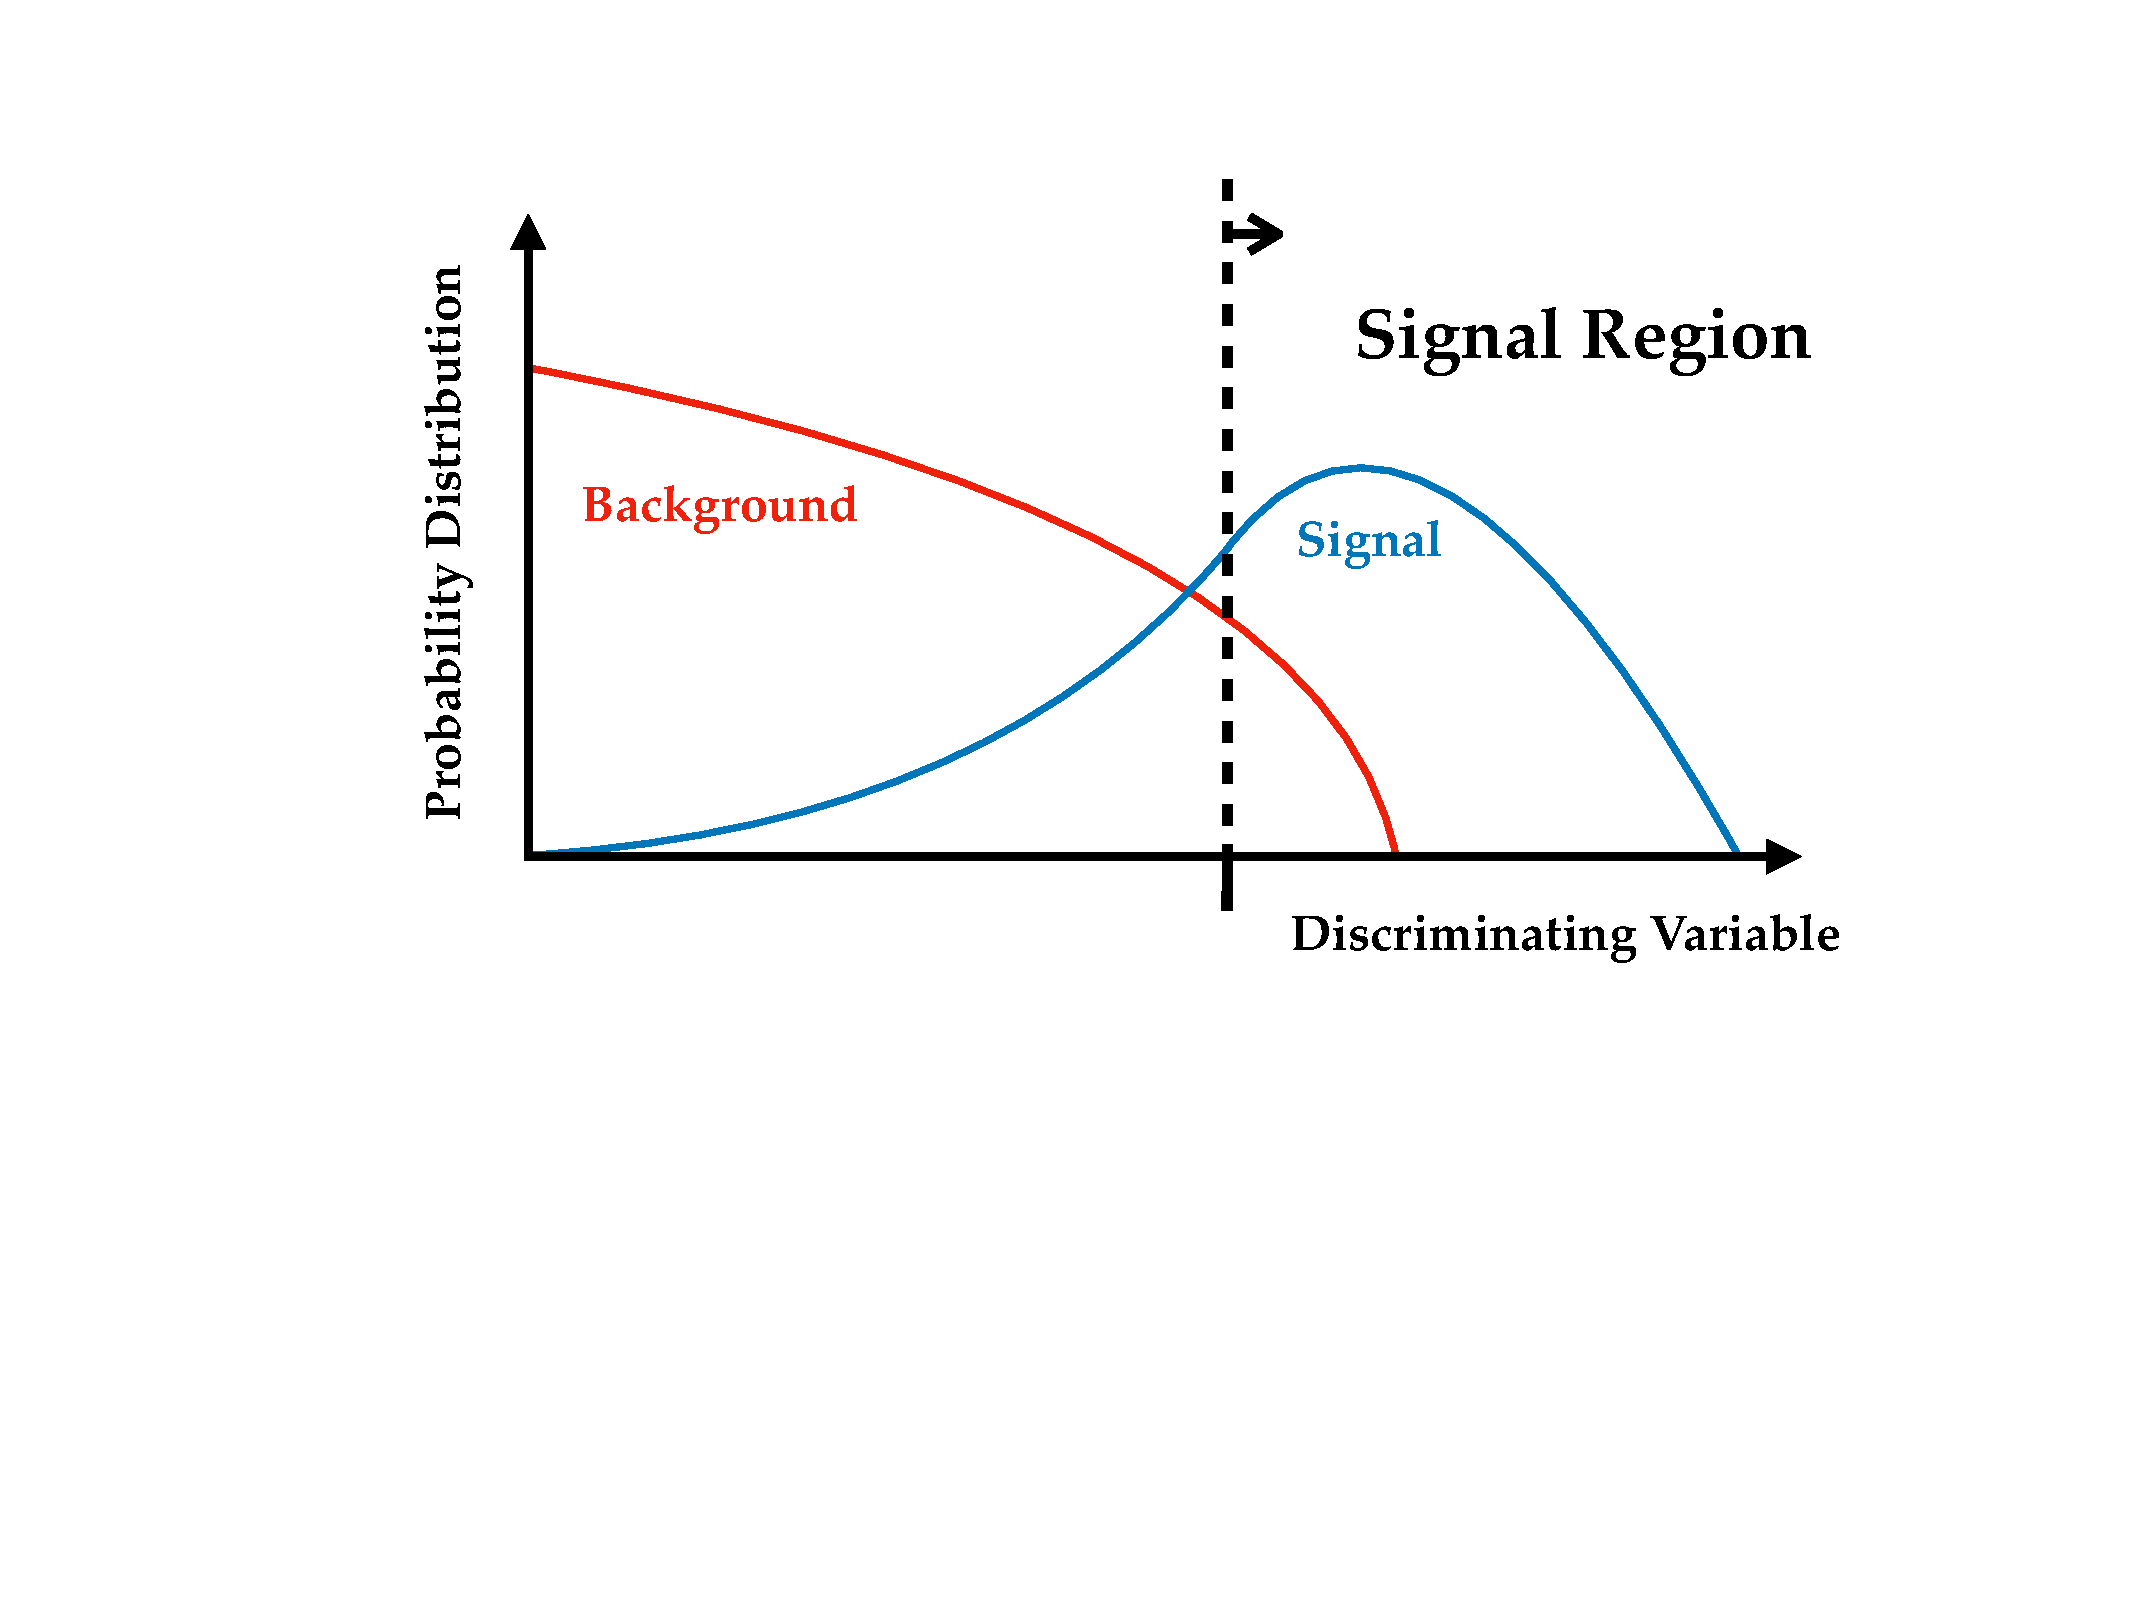
\includegraphics[width=0.65\textwidth]{figures/common_ana/sr_search_vPDF}
        \caption{
            Signal region concept illustrated in the case of a one-dimensional selection
            made on a discriminating kinematic observable.
            The dominant SM background (red) is characterised by typically small values
            of the discriminating variable whereas the signal (blue) has values that extend
            beyond that of the background.
            The signal region in this case is defined by requiring $pp$ collision events
            to have values of the discriminating variable that are larger than
            the value indicated by the dashed vertical line, where the signal purity is
            enhanced.
            The $y$-axis represents the probability distribution of the background and signal
            processes, not their absolute yield for a given range of the quantity on the $x$-axis.
        }
        \label{fig:sr_search_v}
    \end{center}
\end{figure}



%%%%%%%%%%%%%%%%%%%%%%%%%%%%%%%%%%%%%%%%%%%%%%%%%%%%%%%%%%%%%%%%%%%%%%%%%%%%%
% GATHER THE DATA
%%%%%%%%%%%%%%%%%%%%%%%%%%%%%%%%%%%%%%%%%%%%%%%%%%%%%%%%%%%%%%%%%%%%%%%%%%%%%
\FloatBarrier

%%%%%%%%%%%%%%%%%%%%%%%%%%%%%%%%%%%%%%%%%%%%%%%%%%%%%%%%%%%%%%%%%%%%%%%%%%%%%
% THE CONTROL REGION METHOD
%%%%%%%%%%%%%%%%%%%%%%%%%%%%%%%%%%%%%%%%%%%%%%%%%%%%%%%%%%%%%%%%%%%%%%%%%%%%%
\subsection{Background Estimation and the Control Region Method}
\label{sec:control_region_method}

The general principle behind searches for new physics is to define a SR, or a set of SRs,
and then make predictions about how the signal and background behave therein.
Such predictions can then be compared to the data actually recorded by the ATLAS detector
and the statistical procedures described in Section~\ref{sec:stat_hypo} can be used to
make statements about whether or not --- or to what degree --- the data is likely to contain the specified signal.
The emphasis, then, in physics analyses is on the understanding and precise estimation of the backgrounds.
Without being able to properly estimate the contribution of the background processes to the
events observed in the SRs well-defined predictions cannot therein be made, resulting in ineffective
analyses.

The process of estimating the backgrounds in an analysis' SRs is aptly referred to as
\textit{background estimation}.
There are many background estimation methods that are used.
There exist general background estimation techniques, applicable to a wide range of SM processes,
as well as more dedicated estimation techniques that are specific to a smaller subset of
SM processes.
Most rely on the MC simulation of the SM processes, either as the primary source of providing
the prediction of a given SM process in an analysis' SR(s) or secondarily, as a means of providing a
cross-check on or input to a prediction obtained using the observed data obtained in auxiliary measurements as the primary source.
The high levels of accuracy imposed upon the ATLAS MC simulation infrastructure is derived
from the large and dominant role that the MC simulation plays in the background estimation
procedures in almost all analyses performed by the ATLAS experiment.

The same background estimation strategy is used in each of the analyses to be presented in the
present thesis and is as follows.
Once the SRs designed to capture the sought-for signal are defined, MC simulation can be
used to determine the overall contribution of all SM background processes.
In such a way, the MC simulation can be used to understand which SM processes in the SR(s)
are dominant and which are sub-dominant.
The former are those whose relative contribution to the total background prediction
are large and the latter are those for which this quantity is small or negligible.
As illustrated in Figure~\ref{fig:sr_search_v} for the one-dimensional example,
SR(s) are typically defined by events populating the \textit{tails} of discriminating
observables or probe extreme regions of phase space.
%The tails of such observables are regions of low cross-section and
Such regions typically exhibit low cross-section (background rates) and
are regions of phase space for which the underlying theoretical inputs
to the MC may be less well-understood as compared to the bulk of the phase space.
The MC simulation by itself, therefore, may not be able to adequately describe the background
processes in the SRs defined in these regions, failing to describe
either the overall cross-section of specific processes or the actual shape of the discriminating observables' distributions
therein.
The former results in a failure in the overall predicted \textit{rate}, or normalisation, of a specific backgrounds' contribution
to the event yields in the regions
and the latter results in a faulure in predicting the background process' \textit{acceptance}.
%Indeed, the tails of many observables are highly sensitive to theoretical parameters used as
%inputs to the MC simulation process which leads the background estimation being sensitive to these
%parameters.
In order to increase the confidence in the background estimates in such SR(s), the analyses in the present
thesis make use of the so-called \textit{control region method}.
This method is characterised by defining a (set of) region(s) in which there is (are) high purities
of the dominant background process(es).
These regions are referred to as \textit{control regions} (CRs) and are ideally defined using the
same basis of observables used to define the analysis' SRs.
The CRs are defined to be orthogonal to the SRs, meaning that no events that satisfy the requirements of
the SRs populate the CRs.
The observed data in the CRs, which are enriched in a specific background process, are used to derive
factors that correct the cross-section predictions of the MC estimates of the dominant background processes for
which the CRs are defined.
The per-process normalisation corrections, $\mu_p$, can essentially be thought of as those factors
that adjust the process' normalisation in such a way as to cover any discrepancy between the observed
data yield and MC prediction for the process in question:
\begin{align}
    \mu_{p} = \frac{  N_{\text{data}}^{\text{CR}} - \sum\limits_{\substack{i \\ i\ne p}} N_{\text{MC},\,i}^{\text{CR}}} { N_{\text{MC},\,p}^{\text{CR}}},
    \label{eq:mu_fac}
    %\mu = \frac{ \left( N_{\text{obs}}^{\text{CR}} - \sum\limits_{i_{i\ne \text{proc}}} \right)} {4}
\end{align}
where `$p$' indicates the process for which the CR is defined, $N_{\text{data}}^{\text{CR}}$ is the observed
data yield in the CR, and $N_{\text{MC},\,j}^{\text{CR}}$ is the predicted yield in MC for the background
process $j$.
If there is more than one process for which a normalisation correction factor is being derived, and therefore
more than one CR, the normalisation factors are constrained by the process' contribution across all CRs in which
it is present and the expression in Equation~\ref{eq:mu_fac} is expanded into a system of equations,
\begin{align}
    N_{\text{data,sub}}^{\text{CR1}} &= \mu_i N_i^{\text{CR1}} + \mu_j N_j^{\text{CR1}} + ... \\
    N_{\text{data,sub}}^{\text{CR2}} &= \mu_i N_i^{\text{CR2}} + \mu_j N_j^{\text{CR2}} + ... \\
        &\vdots
    \label{eq:mu_fac_expand}
\end{align}
where $N_{\text{data,sub}}^{a}$ is the observed data yield in the region $a$ with the MC predictions
for those processes not having a dedicated  CR subtracted (analogous to the numerator appearing in Equation~\ref{eq:mu_fac}),
$\mu_p$ are the normalisation factors for each process being solved for, and $N_p^{a}$ are the MC predictions
for process $p$ in region $a$.
Each process' dedicated CR ideally exhibits both a high purity of the given process and relatively large
number of events and therefore {\color{red}{too large may indicate large extrapolation}}
is the only CR that has any real constraining power on the process' normalisation correction factor.
If this is true, the expression in Equation~\ref{eq:mu_fac} generally holds true for each process with a
CR, even in the case of multiple CRs and
normalisation factors.

As mentioned above, the CRs are ideally defined using the same basic of kinematic observables
as used in the definition of the SR.
When this is the case, it is more likely that the constructed CRs probe a similar kinematic
phase space as that of the SRs.
It is important that the CRs are kinematically similar to the SRs so that the correction factors
derived in them are representative of the SRs; that is, that the underlying root cause of the
correction is the same in both the CRs, where the corrections are derived, and the SRs, where
the corrections are applied.
If an SR requires high numbers of jets (high event activity), for example, but the CR is defined to have zero
jets (low event activity) then any normalisation correction derived in the CR may be correcting for physics effects
that are not relevant to the phase space probed by the SR.

In addition to the CRs, so-called \textit{validation regions} (VRs) are typically defined.
The VRs are typically kinematically more similar to the SRs, while still maintaining orthogonality
between the CRs and the SRs.
VRs are defined for each CR and allow for one to validate the extrapolation of the CR-derived normalisation
correction for each process in a region more similar to the SR.
The validation is done by comparing the post-corrected MC prediction of the backgrounds to the
observed data in the VRs, ensuring that both the overall normalisation of the backgrounds
agrees with the observed data as well as the overall shape of the relevant observables used
in the definition of the SRs.

\begin{figure}[!htb]
    \begin{center}
        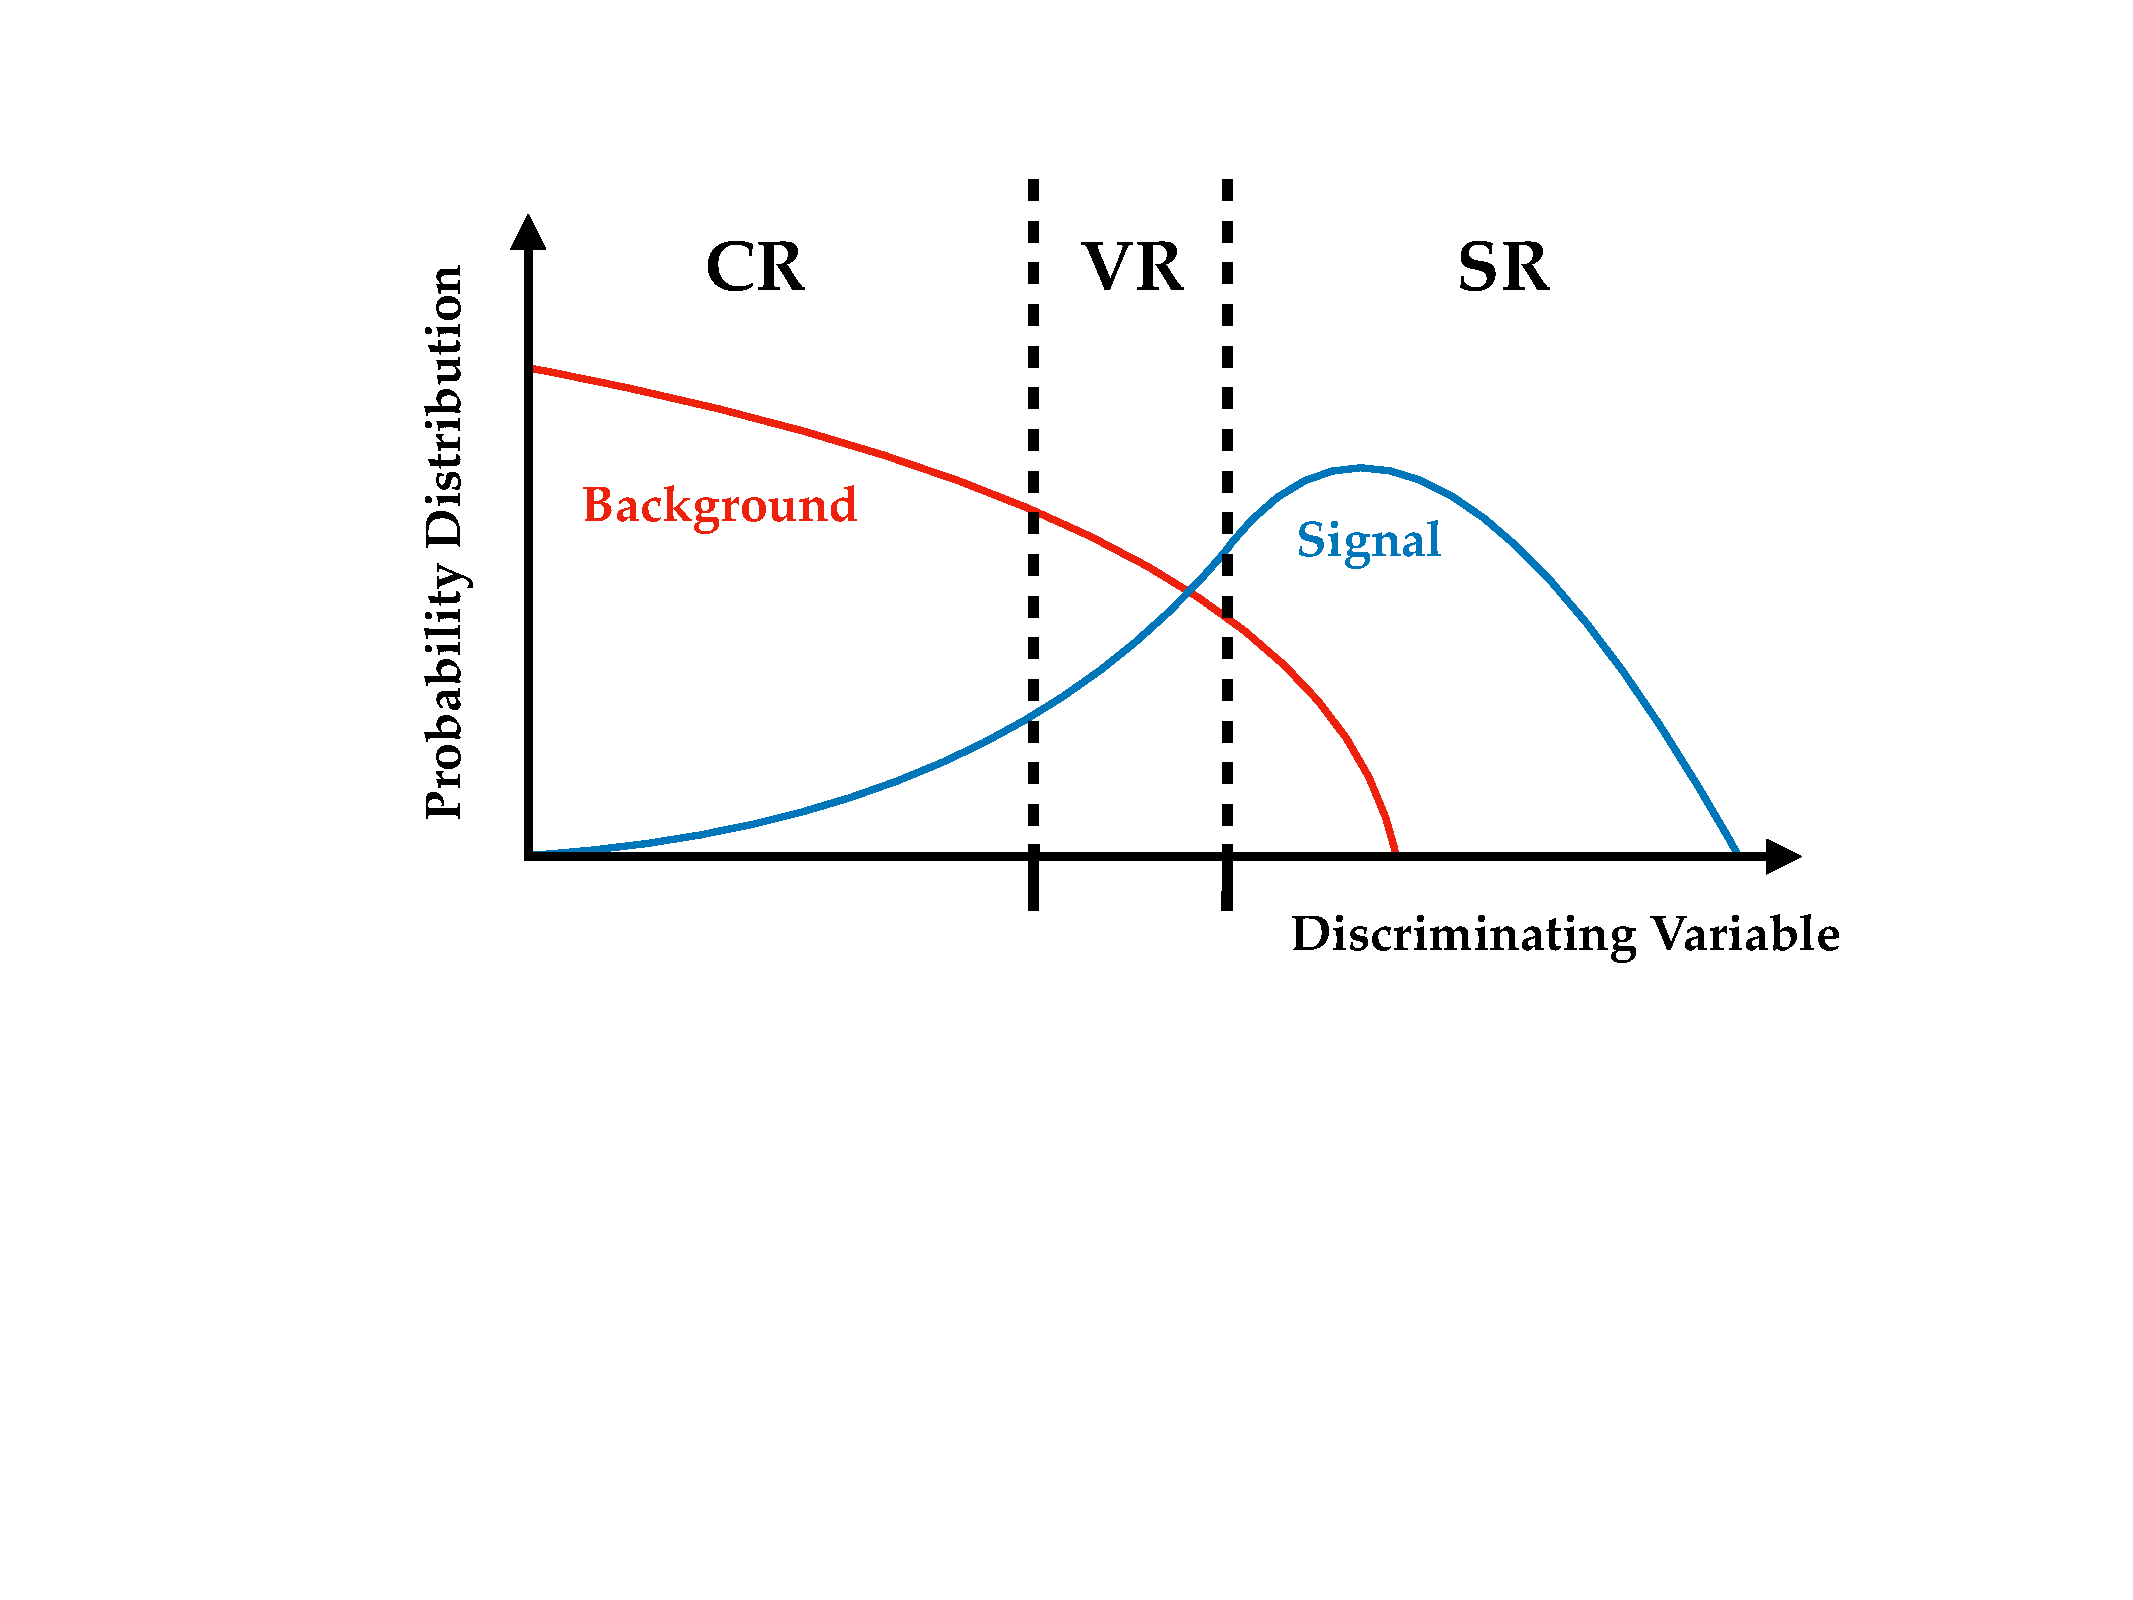
\includegraphics[width=0.65\textwidth]{figures/common_ana/sr_search_v_CRPDF}
        \caption{
            Illustration of the control region method, in the one-dimensional case analogous to that
            presented in Figure~\ref{fig:sr_search_v}.
            The control region (CR) is pure in the background process but is defined kinematically alongside the signal region (SR).
            A validation region (VR), ideally still with high background purity, is defined between the CR and SR and is used to validate
            the extrapolation of the background estimate from the CR to the SR.
            The $y$-axis represents the probability distribution of the background and signal
            processes, not their absolute yield for a given range of the quantity on the $x$-axis.
        }
        \label{fig:sr_search_v_CR}
    \end{center}
\end{figure}

%%%%%%%%%%%%%%%%%%%%%%%%%%%%%%%%%%%%%%%%%%%%%%%%%%%%%%%%%%%%%%%%%%%%%%%%%%%%%
% SYSTEMATIC UNCERTAINTIES
%%%%%%%%%%%%%%%%%%%%%%%%%%%%%%%%%%%%%%%%%%%%%%%%%%%%%%%%%%%%%%%%%%%%%%%%%%%%%
